%% PGFPlots 代码 - 插入到 LaTeX 中直接生成矢量图
%% 需要添加: \usepackage{pgfplots}
%% \pgfplotsset{compat=1.18}

\begin{figure}[t]
\centering
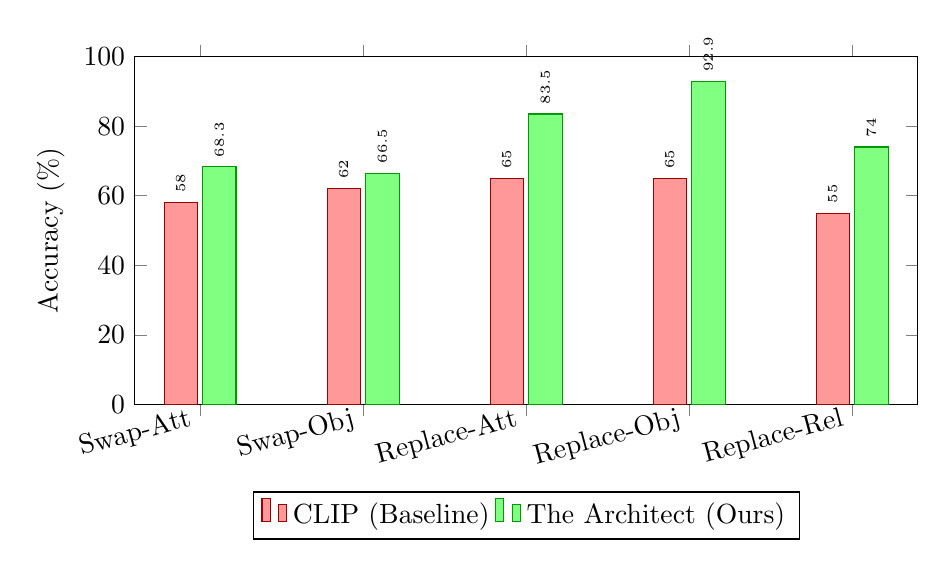
\begin{tikzpicture}
\begin{axis}[
    ybar,
    bar width=12pt,
    width=0.95\linewidth,
    height=6cm,
    ylabel={Accuracy (\%)},
    symbolic x coords={Swap-Att, Swap-Obj, Replace-Att, Replace-Obj, Replace-Rel},
    xtick=data,
    x tick label style={rotate=15, anchor=east},
    ymin=0, ymax=100,
    legend style={at={(0.5,-0.25)}, anchor=north, legend columns=2},
    nodes near coords,
    nodes near coords style={font=\tiny},
    every node near coord/.append style={rotate=90, anchor=west},
]

\addplot[fill=red!40, draw=red!60!black] coordinates {
    (Swap-Att, 58.0)
    (Swap-Obj, 62.0)
    (Replace-Att, 65.0)
    (Replace-Obj, 65.0)
    (Replace-Rel, 55.0)
};
\addplot[fill=green!50, draw=green!60!black] coordinates {
    (Swap-Att, 68.3)
    (Swap-Obj, 66.5)
    (Replace-Att, 83.5)
    (Replace-Obj, 92.9)
    (Replace-Rel, 74.0)
};

\legend{CLIP (Baseline), The Architect (Ours)}
\end{axis}
\end{tikzpicture}
\caption{Comparison with CLIP on SugarCrepe benchmark.}
\label{fig:sugarcrepe}
\end{figure}
